\newpage
\subsection{Caso d'uso UC7: Visualizzazione API}
\label{UC7}
\begin{figure}[ht]
	\centering
	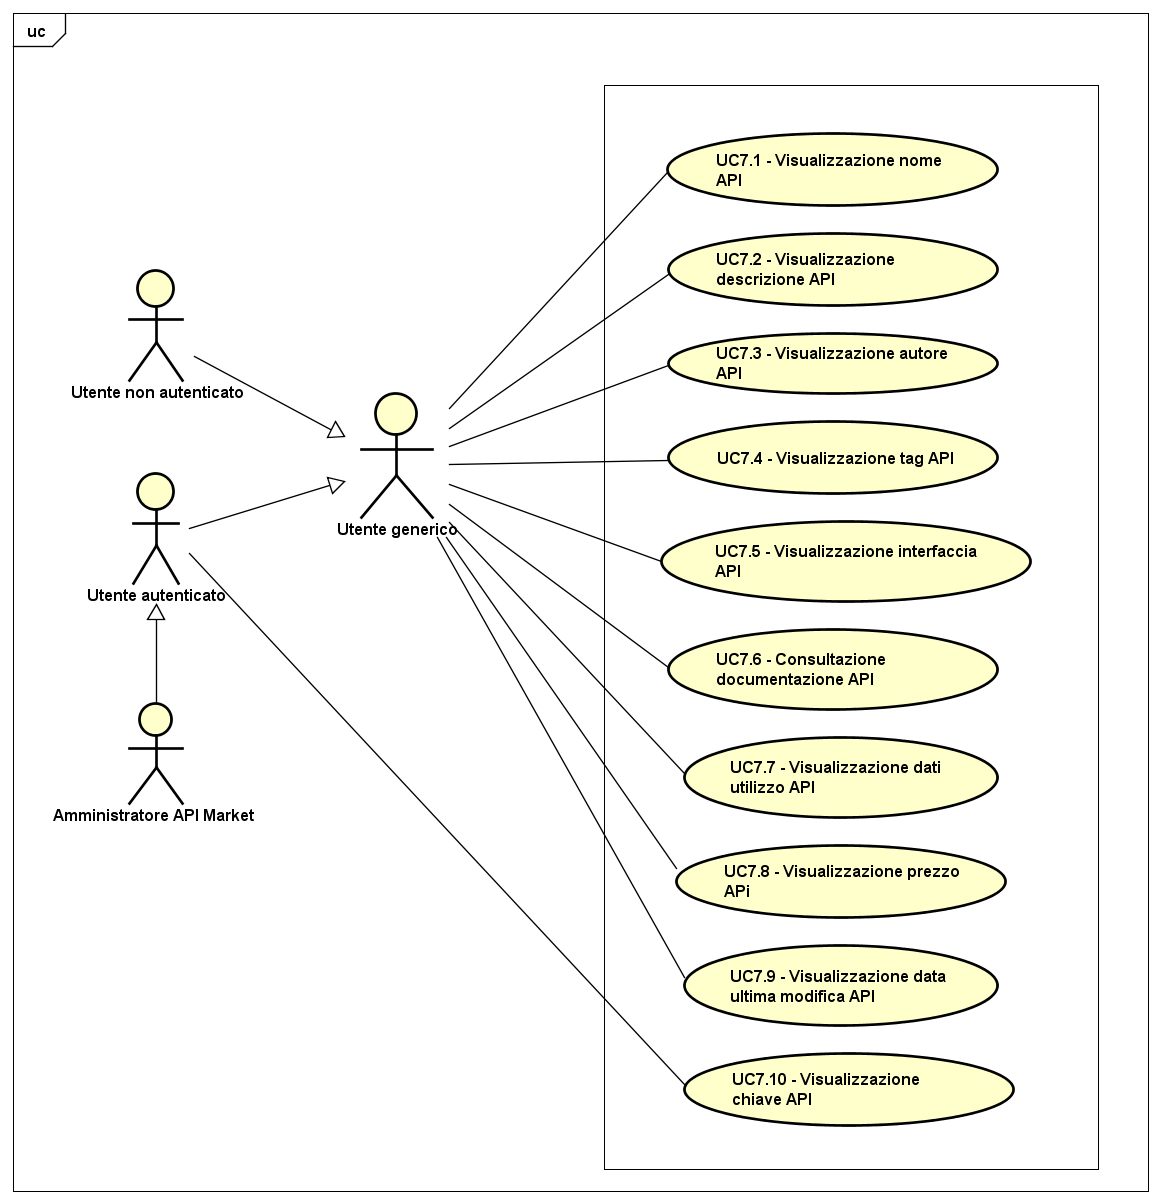
\includegraphics[scale=0.45]{UML/UC7.png}
	\caption{UC7: Visualizzazione API}
\end{figure}

\begin{longtable}{ l | p{11cm}}
	\hline
	\rowcolor{Gray}
	\multicolumn{2}{c}{UC7 - Visualizzazione API}\\
	\hline
	
	 \textbf{Attori} & Utente generico, Utente non autenticato, Utente autenticato, Amministratore API Market \\
	\textbf{Descrizione} & L'attore visualizza i dati relativi ad una API \\
	\textbf{Pre-Condizioni} & L'attore ha selezionato una API tramite un link (ottenuto da una ricerca od altro) e si trova nella sua schermata di visualizzazione \\
	\textbf{Post-Condizioni} & L'attore ha visualizzato la pagina dei dati relativi all'API selezionata \\
	\textbf{Scenario Principale} &
	\begin{enumerate*}[label=(\arabic*.),itemjoin={\newline}]
		\item L'attore può visualizzare il nome dell'API (UC7.1)
		\item L'attore può visualizzare la descrizione dell'API (UC7.2)
		\item L'attore può visualizzare il nome dell'autore dell'API (UC7.3)
		\item L'attore può visualizzare i tag registrati relativi all'API (UC7.4)
		\item L'attore può visualizzare l'interfaccia dell'API (UC7.5)
		\item L'attore può consultare la documentazione dell'API (UC7.6)
		\item L'attore può visualizzare i dati di utilizzo dell'API (UC7.7)
		\item L'attore può visualizzare il prezzo dell'API (UC7.8)
		\item L'utente autenticato può visualizzare la propria chiave API, se la possiede (UC7.9)
		\item L'utente autenticato può acquistare l'API (UC9)
	\end{enumerate*}\\
\end{longtable}


\subsubsection{Caso d'uso UC7.1: Visualizzazione nome API}
\label{UC7_1}

\begin{minipage}{\linewidth}
	\begin{tabular}{ l | p{11cm}}
		\hline
		\rowcolor{Gray}
		\multicolumn{2}{c}{UC7.1 - Visualizzazione nome API} \\
		\hline
		\textbf{Attori} & Utente generico, Utente non autenticato, Utente autenticato, Amministratore API Market \\
		\textbf{Descrizione} & L'attore visualizza nella schermata relativa il nome dell'API \\
		\textbf{Pre-Condizioni} & L'attore si trova nella schermata di visualizzazione API dell'API precedentemente selezionata \\
		\textbf{Post-Condizioni} & L'attore ha visualizzato il nome dell'API selezionata \\
		\textbf{Scenario Principale} & 
		\begin{enumerate*}[label=(\arabic*.),itemjoin={\newline}]
			\item L'attore può visualizzare il nome dell'API selezionata
		\end{enumerate*}\\
	\end{tabular}
\end{minipage}

\subsubsection{Caso d'uso UC7.2: Visualizzazione descrizione API}
\label{UC7_2}

\begin{minipage}{\linewidth}
	\begin{tabular}{ l | p{11cm}}
		\hline
		\rowcolor{Gray}
		\multicolumn{2}{c}{UC7.2 - Visualizzazione descrizione API} \\
		\hline
		\textbf{Attori} & Utente generico, Utente non autenticato, Utente autenticato, Amministratore API Market \\
		\textbf{Descrizione} & L'attore visualizza nella schermata relativa la descrizione dell'API \\
		\textbf{Pre-Condizioni} & L'attore si trova nella schermata di visualizzazione API dell'API precedentemente selezionata \\
		\textbf{Post-Condizioni} & L'attore ha visualizzato la descrizione dell'API selezionata \\
		\textbf{Scenario Principale} & 
		\begin{enumerate*}[label=(\arabic*.),itemjoin={\newline}]
			\item L'attore può visualizzare la descrizione dell'API selezionata
		\end{enumerate*}\\
	\end{tabular}
\end{minipage}

\subsubsection{Caso d'uso UC7.3: Visualizzazione autore API}
\label{UC7_3}

\begin{minipage}{\linewidth}
	\begin{tabular}{ l | p{11cm}}
		\hline
		\rowcolor{Gray}
		\multicolumn{2}{c}{UC7.3 - Visualizzazione autore API} \\
		\hline
		\textbf{Attori} & Utente generico, Utente non autenticato, Utente autenticato, Amministratore API Market \\
		\textbf{Descrizione} & L'attore visualizza nella schermata relativa il nome dell'autore dell'API \\
		\textbf{Pre-Condizioni} & L'attore si trova nella schermata di visualizzazione API dell'API precedentemente selezionata \\
		\textbf{Post-Condizioni} & L'attore ha visualizzato il nome dell'autore per l'API selezionata \\
		\textbf{Scenario Principale} & 
		\begin{enumerate*}[label=(\arabic*.),itemjoin={\newline}]
			\item L'attore può visualizzare il nome dell'autore per l'API selezionata
		\end{enumerate*}\\
	\end{tabular}
\end{minipage}

\subsubsection{Caso d'uso UC7.4: Visualizzazione tag API}
\label{UC7_4}

\begin{minipage}{\linewidth}
	\begin{tabular}{ l | p{11cm}}
		\hline
		\rowcolor{Gray}
		\multicolumn{2}{c}{UC7.4 - Visualizzazione tag API} \\
		\hline
		\textbf{Attori} & Utente generico, Utente non autenticato, Utente autenticato, Amministratore API Market \\
		\textbf{Descrizione} & L'attore visualizza nella schermata relativa i tag assegnati all'API \\
		\textbf{Pre-Condizioni} & L'attore si trova nella schermata di visualizzazione API dell'API precedentemente selezionata \\
		\textbf{Post-Condizioni} & L'attore ha visualizzato i tag assegnati all'API selezionata \\
		\textbf{Scenario Principale} & 
		\begin{enumerate*}[label=(\arabic*.),itemjoin={\newline}]
			\item L'attore può visualizzare i tag assegnati all'API selezionata
		\end{enumerate*}\\
	\end{tabular}
\end{minipage}

\subsubsection{Caso d'uso UC7.5: Visualizzazione interfaccia API}
\label{UC7_5}

\begin{minipage}{\linewidth}
	\begin{tabular}{ l | p{11cm}}
		\hline
		\rowcolor{Gray}
		\multicolumn{2}{c}{UC7.5 - Visualizzazione interfaccia API} \\
		\hline
		\textbf{Attori} & Utente generico, Utente non autenticato, Utente autenticato, Amministratore API Market \\
		\textbf{Descrizione} & L'attore visualizza nella schermata relativa l'interfaccia dell'API \\
		\textbf{Pre-Condizioni} & L'attore si trova nella schermata di visualizzazione API dell'API precedentemente selezionata \\
		\textbf{Post-Condizioni} & L'attore ha visualizzato l'interfaccia dell'API selezionata \\
		\textbf{Scenario Principale} & 
		\begin{enumerate*}[label=(\arabic*.),itemjoin={\newline}]
			\item L'attore può visualizzare l'interfaccia dell'API selezionata
		\end{enumerate*}\\
	\end{tabular}
\end{minipage}

\newpage
\subsubsection{Caso d'uso UC7.6: Consultazione documentazione API}
\label{UC7_6}
\begin{figure}[ht]
	\centering
	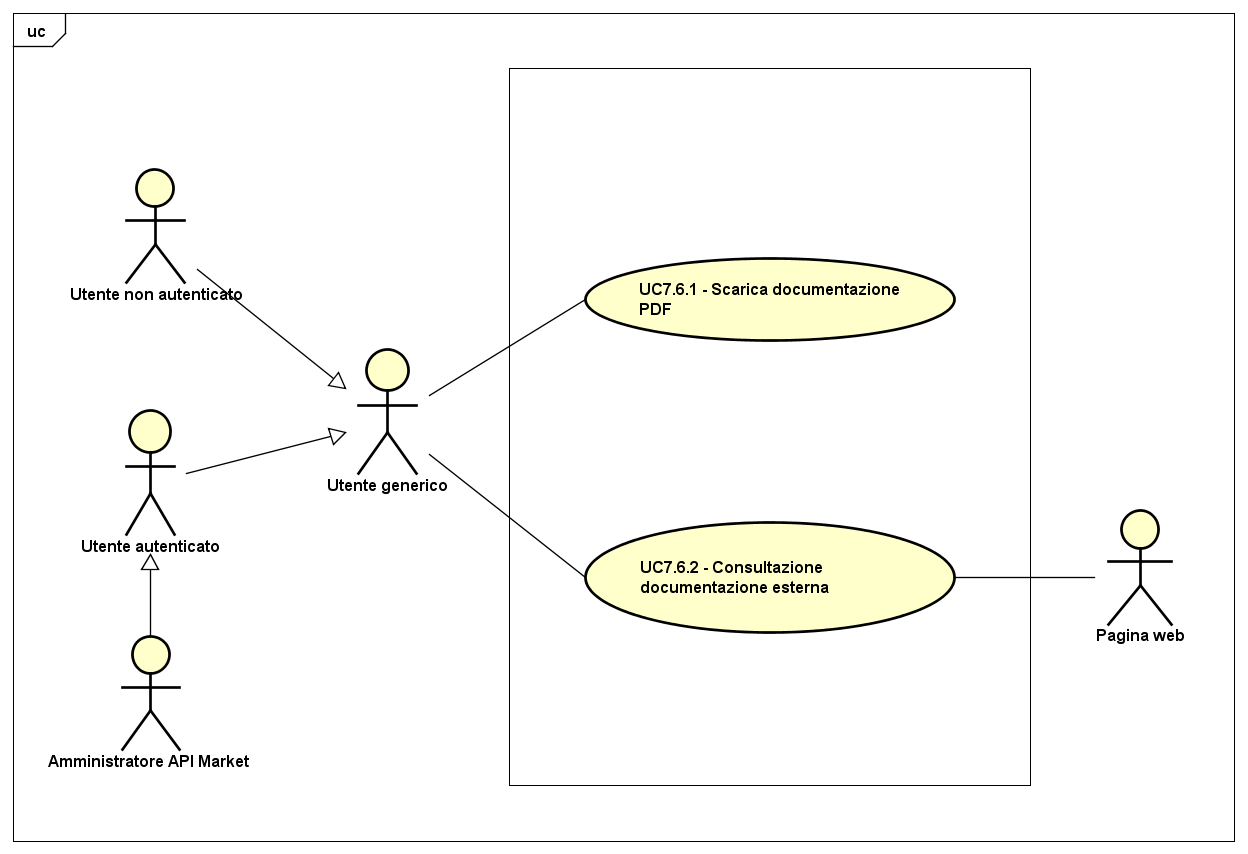
\includegraphics[scale=0.45]{UML/UC7_6.png}
	\caption{UC7.6: Visualizzazione API}
\end{figure}

\begin{minipage}{\linewidth}
	\begin{tabular}{ l | p{11cm}}
		\hline
		\rowcolor{Gray}
		\multicolumn{2}{c}{UC7.6 - Consultazione documentazione API} \\
		\hline
		\textbf{Attori} & Utente generico, Utente non autenticato, Utente autenticato, Amministratore API Market, Pagina web \\
		\textbf{Descrizione} & L'attore consulta la documentazione dell'API \\
		\textbf{Pre-Condizioni} & L'attore si trova nella schermata di visualizzazione API dell'API precedentemente selezionata \\
		\textbf{Post-Condizioni} & L'attore ha consultato la documentazione dell'API selezionata \\
		\textbf{Scenario Principale} & 
		\begin{enumerate*}[label=(\arabic*.),itemjoin={\newline}]
			\item L'attore può consultare la documentazione dell'API selezionata scaricando il file PDF fornito dall'autore (UC7.6.1)
			\item L'attore può consultare la documentazione dell'API selezionata tramite un link esterno fornita dall'autore (UC7.6.2)
		\end{enumerate*}\\
	\end{tabular}
\end{minipage}

\paragraph{Caso d'uso UC7.6.1: Scarica documentazione PDF}
\label{UC7_6_1}

\begin{minipage}{\linewidth}
	\begin{tabular}{ l | p{11cm}}
		\hline
		\rowcolor{Gray}
		\multicolumn{2}{c}{UC7.6.1 - Scarica documentazione PDF} \\
		\hline
		\textbf{Attori} & Utente generico, Utente non autenticato, Utente autenticato, Amministratore API Market \\
		\textbf{Descrizione} & L'attore scarica la documentazione dell'API in formato PDF tramite un link \\
		\textbf{Pre-Condizioni} & L'attore si trova nella schermata relativa alla consultazione della documentazione dell'API \\
		\textbf{Post-Condizioni} & L'attore ha scaricato la documentazione dell'API in formato PDF \\
		\textbf{Scenario Principale} & 
		\begin{enumerate*}[label=(\arabic*.),itemjoin={\newline}]
			\item L'attore può scaricare la documentazione dell'API in formato PDF
		\end{enumerate*}\\
	\end{tabular}
\end{minipage}

\paragraph{Caso d'uso UC7.6.2: Consultazione documentazione esterna}
\label{UC7_6_2}

\begin{minipage}{\linewidth}
	\begin{tabular}{ l | p{11cm}}
		\hline
		\rowcolor{Gray}
		\multicolumn{2}{c}{UC7.6.2 - Consultazione documentazione esterna} \\
		\hline
		\textbf{Attori} & Utente generico, Utente non autenticato, Utente autenticato, Amministratore API Market, Pagina web \\
		\textbf{Descrizione} & L'attore consulta la documentazione dell'API tramite un link esterno fornito dall'autore \\
		\textbf{Pre-Condizioni} & L'attore si trova nella schermata relativa alla consultazione della documentazione dell'API \\
		\textbf{Post-Condizioni} & L'attore ha aperto il link alla documentazione esterna dell'API ed è stato reindirizzato ad una pagina esterna specificata dall'autore dell'API \\
		\textbf{Scenario Principale} & 
		\begin{enumerate*}[label=(\arabic*.),itemjoin={\newline}]
			\item L'attore può consultare la documentazione esterna dell'API aprendo il link ad una pagina esterna specificata dall'autore dell'API
		\end{enumerate*}\\
	\end{tabular}
\end{minipage}

\newpage
\subsubsection{Caso d'uso UC7.7: Visualizzazione dati di utilizzo API}
\label{UC7_7}
\begin{figure}[ht]
	\centering
	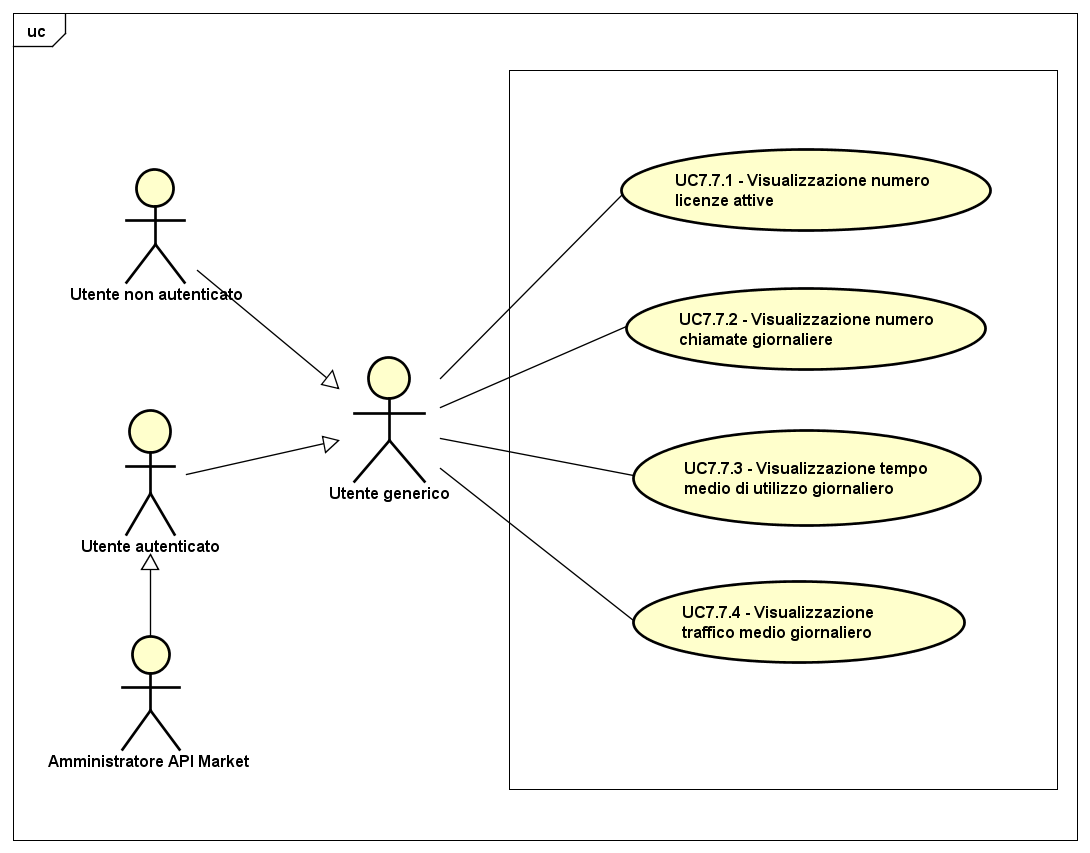
\includegraphics[scale=0.45]{UML/UC7_7.png}
	\caption{UC7.7: Visualizzazione API}
\end{figure}

\begin{minipage}{\linewidth}
	\begin{tabular}{ l | p{11cm}}
		\hline
		\rowcolor{Gray}
		\multicolumn{2}{c}{UC7.7 - Visualizzazione dati di utilizzo API} \\
		\hline
		\textbf{Attori} & Utente generico, Utente non autenticato, Utente autenticato, Amministratore API Market \\
		\textbf{Descrizione} & L'attore visualizza nella schermata relativa i dati di utilizzo dell'API \\
		\textbf{Pre-Condizioni} & L'attore si trova nella schermata di visualizzazione API dell'API precedentemente selezionata \\
		\textbf{Post-Condizioni} & L'attore ha visualizzato i dati di utilizzo dell'API selezionata \\
		\textbf{Scenario Principale} & 
		\begin{enumerate*}[label=(\arabic*.),itemjoin={\newline}]
			\item L'attore può visualizzare il numero di licenze attive per l'API selezionata (UC7.7.1)
			\item L'attore può visualizzare il numero di chiamate giornaliere effettuate all'API selezionata (UC7.7.2)
			\item L'attore può visualizzare il tempo medio di utilizzo giornaliero dell'API selezionata (UC7.7.3)
			\item L'attore può visualizzare il traffico medio giornaliero dell'API selezionata (UC7.7.4)
		\end{enumerate*}\\
	\end{tabular}
\end{minipage}

\paragraph{Caso d'uso UC7.7.1: Visualizzazione numero licenze attive}
\label{UC7_7_1}

\begin{minipage}{\linewidth}
	\begin{tabular}{ l | p{11cm}}
		\hline
		\rowcolor{Gray}
		\multicolumn{2}{c}{UC7.7.1 - Visualizzazione numero licenze attive} \\
		\hline
		\textbf{Attori} & Utente generico, Utente non autenticato, Utente autenticato, Amministratore API Market \\
		\textbf{Descrizione} & L'attore visualizza il numero di licenze attive per l'API selezionata \\
		\textbf{Pre-Condizioni} & L'attore si trova nella schermata di visualizzazione dati di utilizzo API \\
		\textbf{Post-Condizioni} & L'attore ha visualizzato il numero di licenze attive per l'API selezionata \\
		\textbf{Scenario Principale} & 
		\begin{enumerate*}[label=(\arabic*.),itemjoin={\newline}]
			\item L'attore può visualizzare il numero di licenze attive per l'API selezionata
		\end{enumerate*}\\
	\end{tabular}
\end{minipage}

\paragraph{Caso d'uso UC7.7.2: Visualizzazione numero chiamate giornaliere}
\label{UC7_7_2}

\begin{minipage}{\linewidth}
	\begin{tabular}{ l | p{11cm}}
		\hline
		\rowcolor{Gray}
		\multicolumn{2}{c}{UC7.7.2 - Visualizzazione numero chiamate giornaliere} \\
		\hline
		\textbf{Attori} & Utente generico, Utente non autenticato, Utente autenticato, Amministratore API Market \\
		\textbf{Descrizione} & L'attore visualizza il numero di chiamate giornaliere effettuate all'API selezionata \\
		\textbf{Pre-Condizioni} & L'attore si trova nella schermata di visualizzazione dati di utilizzo API \\
		\textbf{Post-Condizioni} & L'attore ha visualizzato il numero di chiamate giornaliere effettuate all'API selezionata \\
		\textbf{Scenario Principale} & 
		\begin{enumerate*}[label=(\arabic*.),itemjoin={\newline}]
			\item L'attore può visualizzare il numero di chiamate giornaliere effettuate all'API selezionata
		\end{enumerate*}\\
	\end{tabular}
\end{minipage}

\paragraph{Caso d'uso UC7.7.3: Visualizzazione tempo medio di utilizzo giornaliero}
\label{UC7_7_3}

\begin{minipage}{\linewidth}
	\begin{tabular}{ l | p{11cm}}
		\hline
		\rowcolor{Gray}
		\multicolumn{2}{c}{UC7.7.3 - Visualizzazione tempo medio di utilizzo giornaliero} \\
		\hline
		\textbf{Attori} & Utente generico, Utente non autenticato, Utente autenticato, Amministratore API Market \\
		\textbf{Descrizione} & L'attore visualizza il tempo medio di utilizzo giornaliero dell'API selezionata \\
		\textbf{Pre-Condizioni} & L'attore si trova nella schermata di visualizzazione dati di utilizzo API \\
		\textbf{Post-Condizioni} & L'attore ha visualizzato il tempo medio di utilizzo giornaliero dell'API selezionata \\
		\textbf{Scenario Principale} & 
		\begin{enumerate*}[label=(\arabic*.),itemjoin={\newline}]
			\item L'attore può visualizzare il tempo medio di utilizzo giornaliero dell'API selezionata
		\end{enumerate*}\\
	\end{tabular}
\end{minipage}

\paragraph{Caso d'uso UC7.7.4: Visualizzazione traffico medio giornaliero}
\label{UC7_7_4}

\begin{minipage}{\linewidth}
	\begin{tabular}{ l | p{11cm}}
		\hline
		\rowcolor{Gray}
		\multicolumn{2}{c}{UC7.7.4 - Visualizzazione traffico medio giornaliero} \\
		\hline
		\textbf{Attori} & Utente generico, Utente non autenticato, Utente autenticato, Amministratore API Market \\
		\textbf{Descrizione} & L'attore visualizza il traffico medio giornaliero dell'API selezionata \\
		\textbf{Pre-Condizioni} & L'attore si trova nella schermata di visualizzazione dati di utilizzo API \\
		\textbf{Post-Condizioni} & L'attore ha visualizzato il traffico medio giornaliero dell'API selezionata \\
		\textbf{Scenario Principale} & 
		\begin{enumerate*}[label=(\arabic*.),itemjoin={\newline}]
			\item L'attore può visualizzare il traffico medio giornaliero dell'API selezionata
		\end{enumerate*}\\
	\end{tabular}
\end{minipage}

\newpage
\subsubsection{Caso d'uso UC7.8: Visualizzazione prezzo API}
\label{UC7_8}
\begin{figure}[ht]
	\centering
	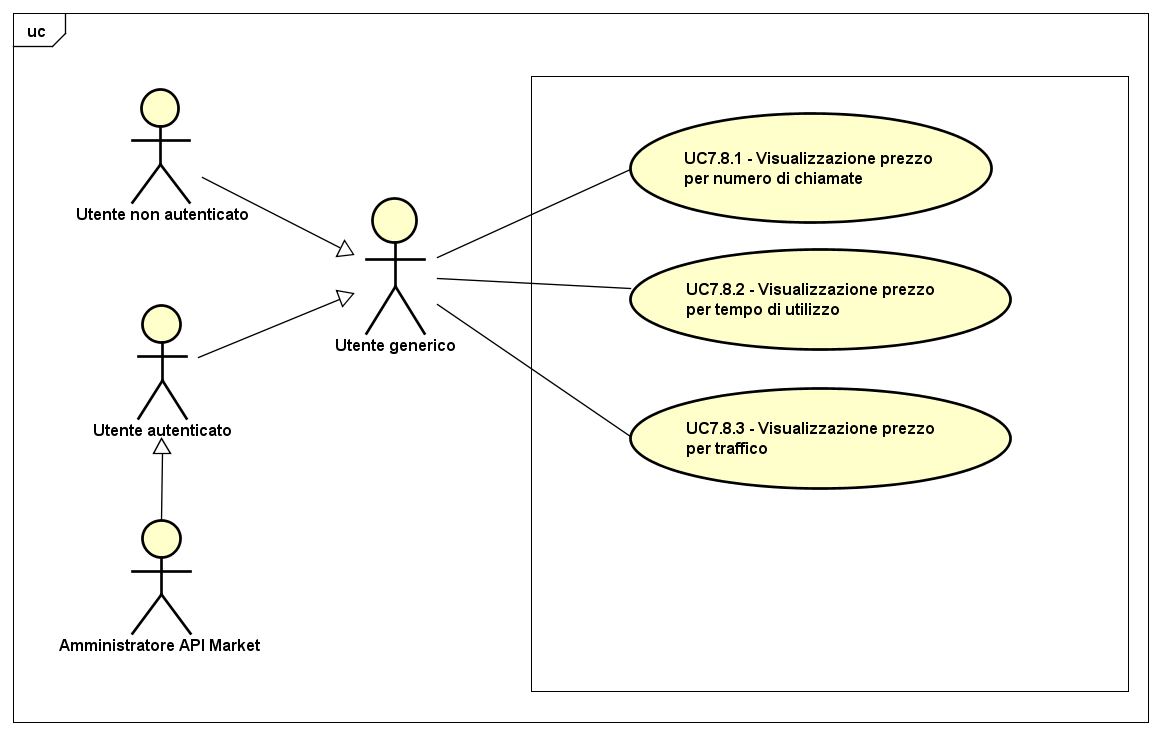
\includegraphics[scale=0.45]{UML/UC7_8.png}
	\caption{UC7.8: Visualizzazione prezzo API}
\end{figure}

\begin{minipage}{\linewidth}
	\begin{tabular}{ l | p{11cm}}
		\hline
		\rowcolor{Gray}
		\multicolumn{2}{c}{UC7.8 - Visualizzazione chiave API} \\
		\hline
		\textbf{Attori} & Utente generico, Utente non autenticato, Utente autenticato, Amministratore API Market \\
		\textbf{Descrizione} & L'attore visualizza nella schermata relativa il prezzo dell'API \\
		\textbf{Pre-Condizioni} & L'attore si trova nella schermata di visualizzazione API dell'API precedentemente selezonata \\
		\textbf{Post-Condizioni} & L'attore ha visualizzato il prezzo dell'API selezionata \\
		\textbf{Scenario Principale} & 
		\begin{enumerate*}[label=(\arabic*.),itemjoin={\newline}]
			\item L'attore può visualizzare il prezzo dell'API per numero di chiamate (UC7.8.1)
			\item L'attore può visualizzare il prezzo dell'API per tempo di utilizzo (UC7.8.2)
			\item L'attore può visualizzare il prezzo dell'API per traffico (UC7.8.3)
		\end{enumerate*}\\
	\end{tabular}
\end{minipage}

\paragraph{Caso d'uso UC7.8.1: Visualizzazione prezzo per numero di chiamate}
\label{UC7_8_1}

\begin{minipage}{\linewidth}
	\begin{tabular}{ l | p{11cm}}
		\hline
		\rowcolor{Gray}
		\multicolumn{2}{c}{UC7.8.1 - Visualizzazione prezzo per numero di chiamate} \\
		\hline
		\textbf{Attori} & Utente generico, Utente non autenticato, Utente autenticato, Amministratore API Market \\
		\textbf{Descrizione} & L'attore visualizza il prezzo per numero di chiamate dell'API \\
		\textbf{Pre-Condizioni} & L'attore si trova nella schermata di visualizzazione API dell'API precedentemente selezionata \\
		\textbf{Post-Condizioni} & L'attore ha visualizzato il prezzo per numero di chiamate dell'API selezionata \\
		\textbf{Scenario Principale} & 
		\begin{enumerate*}[label=(\arabic*.),itemjoin={\newline}]
			\item L'attore può visualizzare il prezzo per numero di chiamate dell'API selezionata
		\end{enumerate*}\\
	\end{tabular}
\end{minipage}

\paragraph{Caso d'uso UC7.8.2: Visualizzazione prezzo per tempo di utilizzo}
\label{UC7_8_2}

\begin{minipage}{\linewidth}
	\begin{tabular}{ l | p{11cm}}
		\hline
		\rowcolor{Gray}
		\multicolumn{2}{c}{UC7.8.2 - Visualizzazione prezzo per tempo di utilizzo} \\
		\hline
		\textbf{Attori} & Utente generico, Utente non autenticato, Utente autenticato, Amministratore API Market \\
		\textbf{Descrizione} & L'attore visualizza il prezzo per tempo di utilizzo dell'API \\
		\textbf{Pre-Condizioni} & L'attore si trova nella schermata di visualizzazione API dell'API precedentemente selezionata \\
		\textbf{Post-Condizioni} & L'attore ha visualizzato il prezzo per tempo di utilizzo dell'API selezionata \\
		\textbf{Scenario Principale} & 
		\begin{enumerate*}[label=(\arabic*.),itemjoin={\newline}]
			\item L'attore può visualizzare il prezzo per tempo di utilizzo dell'API selezionata
		\end{enumerate*}\\
	\end{tabular}
\end{minipage}

\paragraph{Caso d'uso UC7.8.3: Visualizzazione prezzo per traffico}
\label{UC7_8_3}

\begin{minipage}{\linewidth}
	\begin{tabular}{ l | p{11cm}}
		\hline
		\rowcolor{Gray}
		\multicolumn{2}{c}{UC7.8.3 - Visualizzazione prezzo per traffico} \\
		\hline
		\textbf{Attori} & Utente generico, Utente non autenticato, Utente autenticato, Amministratore API Market \\
		\textbf{Descrizione} & L'attore visualizza il prezzo per per traffico dell'API \\
		\textbf{Pre-Condizioni} & L'attore si trova nella schermata di visualizzazione API dell'API precedentemente selezionata \\
		\textbf{Post-Condizioni} & L'attore ha visualizzato il prezzo per per traffico dell'API selezionata \\
		\textbf{Scenario Principale} & 
		\begin{enumerate*}[label=(\arabic*.),itemjoin={\newline}]
			\item L'attore può visualizzare il prezzo per per traffico dell'API selezionata
		\end{enumerate*}\\
	\end{tabular}
\end{minipage}

\subsubsection{Caso d'uso UC7.9: Visualizzazione data ultima modifica API}
\label{UC7_9}

\begin{minipage}{\linewidth}
	\begin{tabular}{ l | p{11cm}}
		\hline
		\rowcolor{Gray}
		\multicolumn{2}{c}{UC7.9 - Visualizzazione data ultima modifica API} \\
		\hline
		\textbf{Attori} & Utente autenticato, Amministratore API Market \\
		\textbf{Descrizione} & L'attore visualizza nella schermata relativa la data dell'ultima modifica effettuata sull'API \\
		\textbf{Pre-Condizioni} & L'attore ha selezionato una API, ne possiede la licenza attiva e si trova nella schermata di visualizzazione API \\
		\textbf{Post-Condizioni} & L'attore ha visualizzato nella schermata relativa la data dell'ultima modifica effettuata sull'API selezionata \\
		\textbf{Scenario Principale} & 
		\begin{enumerate*}[label=(\arabic*.),itemjoin={\newline}]
			\item L'attore può visualizzare nella schermata relativa la data dell'ultima modifica effettuata sull'API selezionata
		\end{enumerate*}\\
	\end{tabular}
\end{minipage}

\subsubsection{Caso d'uso UC7.10: Visualizzazione chiave API}
\label{UC7_10}

\begin{minipage}{\linewidth}
	\begin{tabular}{ l | p{11cm}}
		\hline
		\rowcolor{Gray}
		\multicolumn{2}{c}{UC7.10 - Visualizzazione chiave API} \\
		\hline
		\textbf{Attori} & Utente autenticato, Amministratore API Market \\
		\textbf{Descrizione} & L'attore visualizza nella schermata relativa la propria chiave per l'API \\
		\textbf{Pre-Condizioni} & L'attore ha selezionato una API, ne possiede la licenza attiva e si trova nella schermata di visualizzazione API \\
		\textbf{Post-Condizioni} & L'attore ha visualizzato la propria chiave API per l'API selezionata \\
		\textbf{Scenario Principale} & 
		\begin{enumerate*}[label=(\arabic*.),itemjoin={\newline}]
			\item L'attore può visualizzare la propria chiave API per l'API selezionata
		\end{enumerate*}\\
	\end{tabular}
\end{minipage}